\documentclass{scrartcl}
\usepackage{xcolor, tikz}
\usepackage{pgfplots}
\pgfplotsset{compat=newest}
\pagestyle{empty}
\definecolor{pdg2112}{RGB}{228,26,28}
\definecolor{pdg2212}{RGB}{55,126,184}
\definecolor{pdg1000010020}{RGB}{153,153,153}
\definecolor{pdg1000020040}{RGB}{166,86,40}
\definecolor{pdg11}{RGB}{152,78,163}
\definecolor{pdg1000010030}{RGB}{153,153,153}
\definecolor{pdg22}{RGB}{77,175,74}
\definecolor{pdg1000060120}{RGB}{153,153,153}
\definecolor{pdg1000040090}{RGB}{153,153,153}
\begin{document}
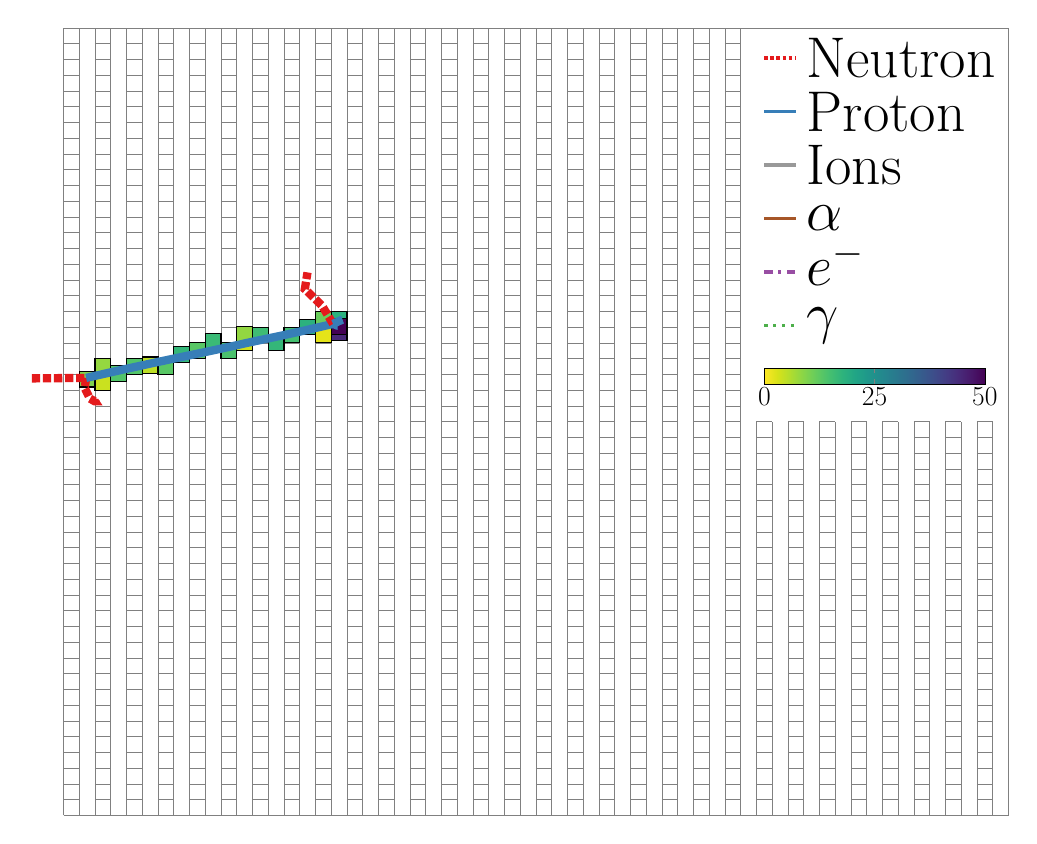
\begin{tikzpicture}[scale=0.4]
\draw[step=0.5,very thin,gray] (21.999000,-12.499) grid (22.500000,0);
\draw[step=0.5,very thin,gray] (22.999000,-12.499) grid (23.500000,0);
\draw[step=0.5,very thin,gray] (23.999000,-12.499) grid (24.500000,0);
\draw[step=0.5,very thin,gray] (24.999000,-12.499) grid (25.500000,0);
\draw[step=0.5,very thin,gray] (25.999000,-12.499) grid (26.500000,0);
\draw[step=0.5,very thin,gray] (26.999000,-12.499) grid (27.500000,0);
\draw[step=0.5,very thin,gray] (27.999000,-12.499) grid (28.500000,0);
\draw[step=0.5,very thin,gray] (28.999000,-12.499) grid (29.500000,0);
\draw[step=0.5,very thin,gray] (-0.001000,-12.499) grid (0.500000,12.499);
\draw[step=0.5,very thin,gray] (0.999000,-12.499) grid (1.500000,12.499);
\draw[step=0.5,very thin,gray] (1.999000,-12.499) grid (2.500000,12.499);
\draw[step=0.5,very thin,gray] (2.999000,-12.499) grid (3.500000,12.499);
\draw[step=0.5,very thin,gray] (3.999000,-12.499) grid (4.500000,12.499);
\draw[step=0.5,very thin,gray] (4.999000,-12.499) grid (5.500000,12.499);
\draw[step=0.5,very thin,gray] (5.999000,-12.499) grid (6.500000,12.499);
\draw[step=0.5,very thin,gray] (6.999000,-12.499) grid (7.500000,12.499);
\draw[step=0.5,very thin,gray] (7.999000,-12.499) grid (8.500000,12.499);
\draw[step=0.5,very thin,gray] (8.999000,-12.499) grid (9.500000,12.499);
\draw[step=0.5,very thin,gray] (9.999000,-12.499) grid (10.500000,12.499);
\draw[step=0.5,very thin,gray] (10.999000,-12.499) grid (11.500000,12.499);
\draw[step=0.5,very thin,gray] (11.999000,-12.499) grid (12.500000,12.499);
\draw[step=0.5,very thin,gray] (12.999000,-12.499) grid (13.500000,12.499);
\draw[step=0.5,very thin,gray] (13.999000,-12.499) grid (14.500000,12.499);
\draw[step=0.5,very thin,gray] (14.999000,-12.499) grid (15.500000,12.499);
\draw[step=0.5,very thin,gray] (15.999000,-12.499) grid (16.500000,12.499);
\draw[step=0.5,very thin,gray] (16.999000,-12.499) grid (17.500000,12.499);
\draw[step=0.5,very thin,gray] (17.999000,-12.499) grid (18.500000,12.499);
\draw[step=0.5,very thin,gray] (18.999000,-12.499) grid (19.500000,12.499);
\draw[step=0.5,very thin,gray] (19.999000,-12.499) grid (20.500000,12.499);
\draw[step=0.5,very thin,gray] (20.999000,-12.499) grid (21.500000,12.499);
\draw[very thin,gray] (0,-12.5) -- (30,-12.5) -- (30,12.5) -- (0,12.5);
\definecolor{tempcolor}{rgb}{0.506271,0.828786,0.300362}\draw[fill=tempcolor,fill opacity=1] (0.500000,1.101024) rectangle (1.000000,1.601024);
\definecolor{tempcolor}{rgb}{0.793760,0.880678,0.120005}\draw[fill=tempcolor,fill opacity=1] (1.000000,1.000000) rectangle (1.500000,1.500000);
\definecolor{tempcolor}{rgb}{0.585678,0.846661,0.249897}\draw[fill=tempcolor,fill opacity=1] (1.000000,1.500000) rectangle (1.500000,2.000000);
\definecolor{tempcolor}{rgb}{0.319809,0.770914,0.411152}\draw[fill=tempcolor,fill opacity=1] (1.500000,1.273730) rectangle (2.000000,1.773730);
\definecolor{tempcolor}{rgb}{0.319809,0.770914,0.411152}\draw[fill=tempcolor,fill opacity=1] (2.000000,1.500000) rectangle (2.500000,2.000000);
\definecolor{tempcolor}{rgb}{0.762373,0.876424,0.137064}\draw[fill=tempcolor,fill opacity=1] (2.500000,1.575120) rectangle (3.000000,2.075120);
\definecolor{tempcolor}{rgb}{0.741388,0.873449,0.149561}\draw[fill=tempcolor,fill opacity=1] (2.500000,1.532795) rectangle (3.000000,2.032795);
\definecolor{tempcolor}{rgb}{0.344074,0.780029,0.397381}\draw[fill=tempcolor,fill opacity=1] (3.000000,1.500000) rectangle (3.500000,2.000000);
\definecolor{tempcolor}{rgb}{0.208030,0.718701,0.472873}\draw[fill=tempcolor,fill opacity=1] (3.500000,1.876917) rectangle (4.000000,2.376917);
\definecolor{tempcolor}{rgb}{0.344074,0.780029,0.397381}\draw[fill=tempcolor,fill opacity=1] (4.000000,2.000000) rectangle (4.500000,2.500000);
\definecolor{tempcolor}{rgb}{0.226397,0.728888,0.462789}\draw[fill=tempcolor,fill opacity=1] (4.500000,2.284508) rectangle (5.000000,2.784508);
\definecolor{tempcolor}{rgb}{0.288921,0.758394,0.428426}\draw[fill=tempcolor,fill opacity=1] (5.000000,2.000000) rectangle (5.500000,2.500000);
\definecolor{tempcolor}{rgb}{0.814576,0.883393,0.110347}\draw[fill=tempcolor,fill opacity=1] (5.500000,2.262994) rectangle (6.000000,2.762994);
\definecolor{tempcolor}{rgb}{0.575563,0.844566,0.256415}\draw[fill=tempcolor,fill opacity=1] (5.500000,2.530487) rectangle (6.000000,3.030487);
\definecolor{tempcolor}{rgb}{0.246070,0.738910,0.452024}\draw[fill=tempcolor,fill opacity=1] (6.000000,2.500000) rectangle (6.500000,3.000000);
\definecolor{tempcolor}{rgb}{0.202219,0.715272,0.476084}\draw[fill=tempcolor,fill opacity=1] (6.500000,2.255038) rectangle (7.000000,2.755038);
\definecolor{tempcolor}{rgb}{0.266941,0.748751,0.440573}\draw[fill=tempcolor,fill opacity=1] (7.000000,2.500000) rectangle (7.500000,3.000000);
\definecolor{tempcolor}{rgb}{0.170948,0.694384,0.493803}\draw[fill=tempcolor,fill opacity=1] (7.500000,2.754088) rectangle (8.000000,3.254088);
\definecolor{tempcolor}{rgb}{0.896320,0.893616,0.096335}\draw[fill=tempcolor,fill opacity=1] (8.000000,2.500000) rectangle (8.500000,3.000000);
\definecolor{tempcolor}{rgb}{0.412913,0.803041,0.357269}\draw[fill=tempcolor,fill opacity=1] (8.000000,3.000000) rectangle (8.500000,3.500000);
\definecolor{tempcolor}{rgb}{0.170948,0.694384,0.493803}\draw[fill=tempcolor,fill opacity=1] (8.500000,3.003902) rectangle (9.000000,3.503902);
\definecolor{tempcolor}{rgb}{0.281412,0.155834,0.469201}\draw[fill=tempcolor,fill opacity=1] (8.500000,2.567302) rectangle (9.000000,3.067302);
\definecolor{tempcolor}{rgb}{0.267004,0.004874,0.329415}\draw[fill=tempcolor,fill opacity=1] (8.500000,2.777215) rectangle (9.000000,3.277215);
\draw[color=pdg2112, line width=3pt, densely dotted] (-1.00669324096109, 1.3734420858139826) -- (-0.006738162041369833, 1.3826598179335394) -- (0.48999999999998634, 1.3872388229386492) -- (0.7173891443857883, 1.3893349293178554);
\draw[color=pdg1000040090, line width=3pt, solid] (0.7173891443857883, 1.3893349293178554);
\draw[color=pdg2112, line width=3pt, densely dotted] (0.7173891443857883, 1.3893349293178554) -- (0.6734613311798284, 1.0644324335910056) -- (0.8415890175877394, 0.7301967529220657) -- (0.9900000000000091, 0.6472200924246885) -- (0.9920000000000073, 0.6472222708494053) -- (0.9899999999999863, 0.6501789919485493) -- (0.984608644838113, 0.6581493587285779) -- (0.9900000000000319, 0.6795091159334969) -- (0.9970000000000028, 0.698426789226152) -- (1.0029999999999972, 0.7146419377627786) -- (1.0080000000000156, 0.7281545615433187) -- (1.0183097534390981, 0.7560169254417064) -- (1.0290791223689666, 0.7585367123761688) -- (1.0100000000000136, 0.6665783660197487) -- (1.0079999999999927, 0.6569386829589476) -- (1.0032703146674067, 0.634142349167511);
\draw[color=pdg2212, line width=3pt, solid] (0.9829847097347738, 0.660550120320416);
\draw[color=pdg2212, line width=3pt, solid] (0.9932187841252471, 0.6454204684801993);
\draw[color=pdg1000060120, line width=3pt, solid] (0.8415890175877394, 0.7301967529220657);
\draw[color=pdg2212, line width=3pt, solid] (0.6734613311798284, 1.0644324335910056);
\draw[color=pdg1000010020, line width=3pt, solid] (0.7173891443857883, 1.3893349293178554);
\draw[color=pdg2212, line width=3pt, solid] (0.7173891443857883, 1.3893349293178554) -- (0.9900000000000091, 1.4506833398555448) -- (1.1632197626584229, 1.49) -- (1.1942697495283028, 1.4969999999999999) -- (1.2207140051000578, 1.5030000000000001) -- (1.242750884743191, 1.5080000000000002) -- (1.490000000000009, 1.5640672706141527) -- (1.9899999999999864, 1.6761719335988854) -- (2.490000000000009, 1.7850069047147894) -- (2.695596926159328, 1.8301894227219475) -- (2.7080254228643073, 1.8328874639495463) -- (2.739465324548064, 1.839654047746242) -- (2.7773076210045473, 1.8478657865876276) -- (2.8088428680516473, 1.8547089022887822) -- (2.821437325219904, 1.8574534350674834) -- (2.9899999999999864, 1.893751923667864) -- (3.443663413637182, 1.9899999999999998) -- (3.477326501465586, 1.9969999999999999) -- (3.5029999999999974, 2.002333396269141) -- (3.811629359093513, 2.0664281625328957) -- (3.9077899655570945, 2.086405006619877) -- (3.9899999999999864, 2.1036254191317756) -- (4.489999999999986, 2.208322086432804) -- (4.693120399753434, 2.2517302491791824) -- (4.990000000000009, 2.3152916294630743) -- (5.490000000000009, 2.4243908631546636) -- (5.766954861296199, 2.4869090302137424) -- (5.779021639303596, 2.489644999074304) -- (5.809412387812131, 2.4965059838742385) -- (5.847674993342617, 2.504612255303326) -- (5.879560497951343, 2.5113674814942324) -- (5.892268477789298, 2.51406586587853) -- (5.990000000000009, 2.534828298116479) -- (6.490000000000009, 2.641114159847306) -- (6.989999999999986, 2.7460965867232163) -- (7.490000000000009, 2.85632823190296) -- (7.990000000000009, 2.971310096566704) -- (8.068621710743718, 2.99) -- (8.09858096587161, 2.9969999999999994) -- (8.124482577279924, 3.003) -- (8.146067253453543, 3.008) -- (8.490000000000009, 3.0882497762164265) -- (8.557853148437289, 3.1039694009427867);
\draw[color=pdg1000010030, line width=3pt, solid] (8.557853148437289, 3.1039694009427867) -- (8.568697139626602, 3.110164620866615) -- (8.577419838161063, 3.1149907832892922);
\draw[color=pdg2112, line width=3pt, densely dotted] (8.557853148437289, 3.1039694009427867) -- (8.510000000000014, 3.1828616996467742) -- (8.497000000000003, 3.2042939338182976) -- (8.323701274788254, 3.4899999999999998) -- (8.20753516759505, 3.6815153240120444) -- (8.010000000000014, 3.8740120610932225) -- (7.714877289802007, 4.161607224239712) -- (7.661440943036905, 4.2069028368061385) -- (7.745921488240174, 4.738391032736295);
\draw[color=pdg2212, line width=3pt, solid] (7.745921488240174, 4.738391032736295);
\draw[color=pdg2212, line width=3pt, solid] (7.714877289802007, 4.161607224239712);
\draw[color=pdg2212, line width=3pt, solid] (8.557853148437289, 3.1039694009427867);
\draw[color=pdg1000020040, line width=3pt, solid] (8.557853148437289, 3.1039694009427867);
\draw[color=pdg2212, line width=3pt, solid] (8.557853148437289, 3.1039694009427867) -- (8.572799522980722, 3.0990398146561544) -- (8.604623413846161, 3.087671222525343) -- (8.626336492841528, 3.0790780264774966) -- (8.642984493931612, 3.0705625729625456) -- (8.655986287729593, 3.0640308665540075) -- (8.667301230402927, 3.0587754963888685) -- (8.67686729515026, 3.0547183264916304) -- (8.683377013020413, 3.052738349530628) -- (8.686950541087299, 3.0515941059898877) -- (8.693828237680282, 3.049578053378613) -- (8.696422264844022, 3.0491875588919943) -- (8.698557319961855, 3.0492011869962763);
\draw[color=pdg1000010020, line width=3pt, solid] (8.557853148437289, 3.1039694009427867);
\draw[color=pdg2212, line width=3pt, solid] (8.557853148437289, 3.1039694009427867) -- (8.625506551066337, 3.136366684727576) -- (8.679096776290043, 3.1611909480318405) -- (8.72097552580783, 3.1810343718521965) -- (8.754678440838735, 3.1963025082171503) -- (8.781641304622644, 3.2078764152018087) -- (8.803653708578532, 3.216735048965382) -- (8.820947843256045, 3.2240515017964753) -- (8.834184369697596, 3.2300454035790254) -- (8.844472411009473, 3.2346929757071288) -- (8.852669874211665, 3.2381104339791067) -- (8.859476990893677, 3.24048700952376);
\draw[color=pdg11, line width=3pt, dashdotted] (4.693120399753434, 2.2517302491791824);
\draw[color=pdg11, line width=3pt, dashdotted] (3.9077899655570945, 2.086405006619877);
\draw[color=pdg11, line width=3pt, dashdotted] (3.811629359093513, 2.0664281625328957);
\draw[color=pdg2112, very thick, densely dotted] (22.25,11.550000) -- (23.25,11.550000) node [right,black] {\huge{Neutron}};
\draw[color=pdg2212, very thick, solid] (22.25,9.850000) -- (23.25,9.850000) node [right,black] {\huge{Proton}};
\draw[color=pdg1000010020, very thick, solid] (22.25,8.150000) -- (23.25,8.150000) node [right,black] {\huge{Ions}};
\draw[color=pdg1000020040, very thick, solid] (22.25,6.450000) -- (23.25,6.450000) node [right,black] {\huge{$\alpha$}};
\draw[color=pdg11, very thick, dashdotted] (22.25,4.750000) -- (23.25,4.750000) node [right,black] {\huge{$e^-_{\vphantom{-}}$}};
\draw[color=pdg22, very thick, dotted] (22.25,3.050000) -- (23.25,3.050000) node [right,black] {\huge{$\gamma$}};
\begin{axis}[%
    at={(22.25cm,2cm)}, %4.75
    hide axis,
    scale only axis,
    height=0pt,
    width=0pt,
    colormap={reverse viridis}{
       indices of colormap={
       \pgfplotscolormaplastindexof{viridis},...,0 of viridis}
    },
    colorbar horizontal,
    point meta min=0,
    point meta max=50,
    label style={font=\Huge},
    tick label style={font=\Huge},
    colorbar style={
       width=7cm,
       xtick={50, 25, 0},
    }]
\end{axis}
\end{tikzpicture}
\end{document}
